\section{Server Class Reference}
\label{classServer}\index{Server@{Server}}
{\tt \#include $<$server.h$>$}

Inheritance diagram for Server:\nopagebreak
\begin{figure}[H]
\begin{center}
\leavevmode
\includegraphics[width=97pt]{classServer__inherit__graph}
\end{center}
\end{figure}
Collaboration diagram for Server:\nopagebreak
\begin{figure}[H]
\begin{center}
\leavevmode
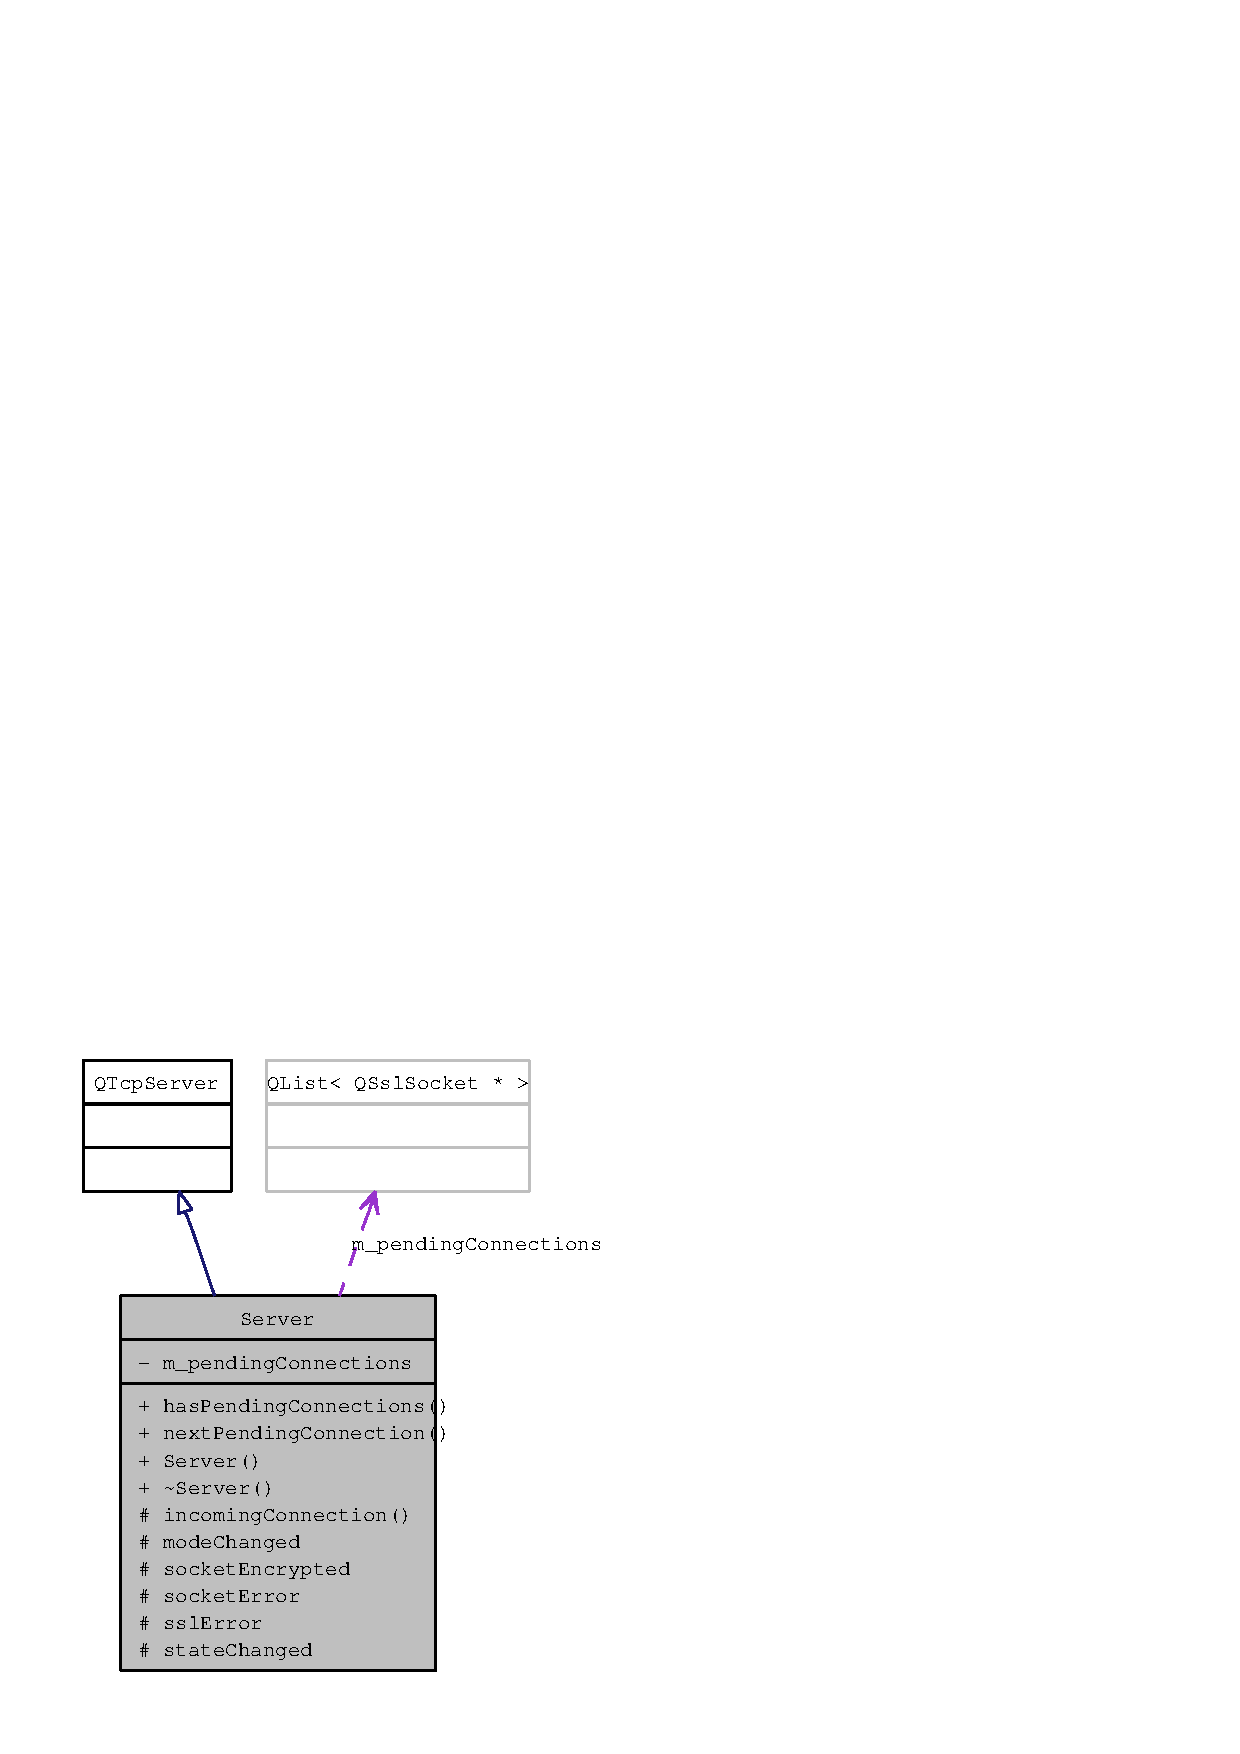
\includegraphics[width=144pt]{classServer__coll__graph}
\end{center}
\end{figure}
\subsection*{Public Member Functions}
\begin{CompactItemize}
\item 
virtual bool {\bf hasPendingConnections} () const 
\item 
virtual QTcpSocket $\ast$ {\bf nextPendingConnection} ()
\item 
{\bf Server} ({\bf QObject} $\ast$parent=0)
\item 
virtual {\bf $\sim$Server} ()
\end{CompactItemize}
\subsection*{Protected Slots}
\begin{CompactItemize}
\item 
void {\bf modeChanged} (QSslSocket::SslMode mode)
\item 
void {\bf socketEncrypted} ()
\item 
void {\bf socketError} (QAbstractSocket::SocketError)
\item 
void {\bf sslError} (const QList$<$ QSslError $>$ \&errors)
\item 
void {\bf stateChanged} (QAbstractSocket::SocketState socketState)
\end{CompactItemize}
\subsection*{Protected Member Functions}
\begin{CompactItemize}
\item 
virtual void {\bf incomingConnection} (int socketDescriptor)
\end{CompactItemize}
\subsection*{Private Attributes}
\begin{CompactItemize}
\item 
QList$<$ QSslSocket $\ast$ $>$ {\bf m\_\-pendingConnections}
\end{CompactItemize}


\subsection{Detailed Description}


Definition at line 8 of file server.h.

\subsection{Constructor \& Destructor Documentation}
\index{Server@{Server}!Server@{Server}}
\index{Server@{Server}!Server@{Server}}
\subsubsection{\setlength{\rightskip}{0pt plus 5cm}Server::Server ({\bf QObject} $\ast$ {\em parent} = {\tt 0})}\label{classServer_1950ac036d86af898428d7ba39bbf048}




Definition at line 34 of file server.cpp.

References certificate(), and key().

\begin{Code}\begin{verbatim}34                               : QTcpServer(parent)
35 {
36     if (key.isNull())
37         qDebug() << "SSL key is null";
38     if (certificate.isNull())
39         qDebug() << "SSL cert is null";
40 }
\end{verbatim}
\end{Code}




Here is the call graph for this function:\nopagebreak
\begin{figure}[H]
\begin{center}
\leavevmode
\includegraphics[width=116pt]{classServer_1950ac036d86af898428d7ba39bbf048_cgraph}
\end{center}
\end{figure}
\index{Server@{Server}!~Server@{$\sim$Server}}
\index{~Server@{$\sim$Server}!Server@{Server}}
\subsubsection{\setlength{\rightskip}{0pt plus 5cm}Server::$\sim$Server ()\hspace{0.3cm}{\tt  [virtual]}}\label{classServer_4b3aa2579cb1c8cd1d069582c14d0fa6}




Definition at line 42 of file server.cpp.

References m\_\-pendingConnections.

\begin{Code}\begin{verbatim}43 {
44     foreach(QSslSocket* s, m_pendingConnections) {
45         s->deleteLater();
46     }
47     m_pendingConnections.clear();
48 }
\end{verbatim}
\end{Code}




\subsection{Member Function Documentation}
\index{Server@{Server}!hasPendingConnections@{hasPendingConnections}}
\index{hasPendingConnections@{hasPendingConnections}!Server@{Server}}
\subsubsection{\setlength{\rightskip}{0pt plus 5cm}bool Server::hasPendingConnections () const\hspace{0.3cm}{\tt  [virtual]}}\label{classServer_fd20de8e190f9d837b1350ca6ffde81a}




Definition at line 50 of file server.cpp.

References m\_\-pendingConnections.

\begin{Code}\begin{verbatim}51 {
52     return m_pendingConnections.count() != 0;
53 }
\end{verbatim}
\end{Code}


\index{Server@{Server}!incomingConnection@{incomingConnection}}
\index{incomingConnection@{incomingConnection}!Server@{Server}}
\subsubsection{\setlength{\rightskip}{0pt plus 5cm}void Server::incomingConnection (int {\em socketDescriptor})\hspace{0.3cm}{\tt  [protected, virtual]}}\label{classServer_48091e8b382412a1f63f05f4cc0ad599}




Definition at line 62 of file server.cpp.

References certificate(), key(), modeChanged(), socketEncrypted(), socketError(), sslError(), and stateChanged().

\begin{Code}\begin{verbatim}63 {
64     qDebug() << "Incoming connection";
65     QSslSocket* socket = new QSslSocket;
66     connect(socket, SIGNAL(encrypted()),
67             this, SLOT(socketEncrypted()));
68     connect(socket, SIGNAL(sslErrors(QList<QSslError>)),
69             this, SLOT(sslError(QList<QSslError>)));
70     connect(socket, SIGNAL(error(QAbstractSocket::SocketError)),
71             this, SLOT(socketError(QAbstractSocket::SocketError)));
72     connect(socket, SIGNAL(stateChanged(QAbstractSocket::SocketState)),
73             this, SLOT(stateChanged(QAbstractSocket::SocketState)));
74     connect(socket, SIGNAL(modeChanged(QSslSocket::SslMode)),
75             this, SLOT(modeChanged(QSslSocket::SslMode)));
76     socket->setPrivateKey(key);
77     socket->setLocalCertificate(certificate);
78     if (socket->setSocketDescriptor(socketDescriptor)) {
79         socket->startServerEncryption();
80         qDebug() << "Started server encryption";
81     } else {
82         qDebug() << "Could not set socket descriptor!";
83         socket->deleteLater();
84     }
85 }
\end{verbatim}
\end{Code}




Here is the call graph for this function:\nopagebreak
\begin{figure}[H]
\begin{center}
\leavevmode
\includegraphics[width=149pt]{classServer_48091e8b382412a1f63f05f4cc0ad599_cgraph}
\end{center}
\end{figure}
\index{Server@{Server}!modeChanged@{modeChanged}}
\index{modeChanged@{modeChanged}!Server@{Server}}
\subsubsection{\setlength{\rightskip}{0pt plus 5cm}void Server::modeChanged (QSslSocket::SslMode {\em mode})\hspace{0.3cm}{\tt  [protected, slot]}}\label{classServer_723b672f1a66356d8a3c929ed1e98ea2}




Definition at line 87 of file server.cpp.

Referenced by incomingConnection().

\begin{Code}\begin{verbatim}88 {
89     qDebug() << mode;
90 }
\end{verbatim}
\end{Code}


\index{Server@{Server}!nextPendingConnection@{nextPendingConnection}}
\index{nextPendingConnection@{nextPendingConnection}!Server@{Server}}
\subsubsection{\setlength{\rightskip}{0pt plus 5cm}QTcpSocket $\ast$ Server::nextPendingConnection ()\hspace{0.3cm}{\tt  [virtual]}}\label{classServer_5875629f158160cbeb4b2c20dfe51d75}




Definition at line 55 of file server.cpp.

References m\_\-pendingConnections.

\begin{Code}\begin{verbatim}56 {
57     QTcpSocket*s = m_pendingConnections.takeFirst();
58     s->disconnect();
59     return s;
60 }
\end{verbatim}
\end{Code}


\index{Server@{Server}!socketEncrypted@{socketEncrypted}}
\index{socketEncrypted@{socketEncrypted}!Server@{Server}}
\subsubsection{\setlength{\rightskip}{0pt plus 5cm}void Server::socketEncrypted ()\hspace{0.3cm}{\tt  [protected, slot]}}\label{classServer_17ef0c2d5e62f72698a1fbcf37ca0d16}




Definition at line 113 of file server.cpp.

References m\_\-pendingConnections.

Referenced by incomingConnection().

\begin{Code}\begin{verbatim}114 {
115     qDebug() << "socket encrypted";
116     QSslSocket* socket = qobject_cast<QSslSocket*>(sender());
117     if (socket) {
118         qDebug() << "Socket go!";
119         m_pendingConnections << socket;
120         emit newConnection();
121     }
122 }
\end{verbatim}
\end{Code}


\index{Server@{Server}!socketError@{socketError}}
\index{socketError@{socketError}!Server@{Server}}
\subsubsection{\setlength{\rightskip}{0pt plus 5cm}void Server::socketError (QAbstractSocket::SocketError {\em e})\hspace{0.3cm}{\tt  [protected, slot]}}\label{classServer_316c33865d07fee74e6b9520a26a243a}




Definition at line 108 of file server.cpp.

Referenced by incomingConnection().

\begin{Code}\begin{verbatim}109 {
110     qDebug() << e;
111 }
\end{verbatim}
\end{Code}


\index{Server@{Server}!sslError@{sslError}}
\index{sslError@{sslError}!Server@{Server}}
\subsubsection{\setlength{\rightskip}{0pt plus 5cm}void Server::sslError (const QList$<$ QSslError $>$ \& {\em errors})\hspace{0.3cm}{\tt  [protected, slot]}}\label{classServer_87fd0cda05a134e8baad67905e4b371b}




Definition at line 97 of file server.cpp.

Referenced by incomingConnection().

\begin{Code}\begin{verbatim}98 {
99     qDebug() << "SSL ERROR";
100     foreach(QSslError e, errors) {
101         qDebug() << e.error() << e.errorString();
102         if (e.error() == QSslError::NoPeerCertificate) {
103             qobject_cast<QSslSocket*>(sender())->ignoreSslErrors();
104         }
105     }
106 }
\end{verbatim}
\end{Code}


\index{Server@{Server}!stateChanged@{stateChanged}}
\index{stateChanged@{stateChanged}!Server@{Server}}
\subsubsection{\setlength{\rightskip}{0pt plus 5cm}void Server::stateChanged (QAbstractSocket::SocketState {\em socketState})\hspace{0.3cm}{\tt  [protected, slot]}}\label{classServer_918bc8cfac493ef59184003bd67219f4}




Definition at line 92 of file server.cpp.

Referenced by incomingConnection().

\begin{Code}\begin{verbatim}93 {
94     qDebug() << socketState;
95 }
\end{verbatim}
\end{Code}




\subsection{Member Data Documentation}
\index{Server@{Server}!m_pendingConnections@{m\_\-pendingConnections}}
\index{m_pendingConnections@{m\_\-pendingConnections}!Server@{Server}}
\subsubsection{\setlength{\rightskip}{0pt plus 5cm}QList$<$QSslSocket$\ast$$>$ {\bf Server::m\_\-pendingConnections}\hspace{0.3cm}{\tt  [private]}}\label{classServer_293548423c35db7e0499696fa262ae95}




Definition at line 28 of file server.h.

Referenced by hasPendingConnections(), nextPendingConnection(), socketEncrypted(), and $\sim$Server().

The documentation for this class was generated from the following files:\begin{CompactItemize}
\item 
{\bf server.h}\item 
{\bf server.cpp}\end{CompactItemize}
